\documentclass{article}
\usepackage{geometry}\geometry{top=.50cm,left=1.cm,right=1.0cm,bottom=.5cm,centering,dvips}
\usepackage{color}
\usepackage[usenames,dvipsnames]{xcolor}
\usepackage{shadow}
\usepackage{kpfonts}
\usepackage{enumitem}
\usepackage{lastpage}
\usepackage{bm}
\usepackage{verbatim}
\usepackage{graphicx}
\usepackage{hyperref}
\hypersetup{colorlinks=true,linkcolor=OliveGreen,citecolor=blue,filecolor=blue,urlcolor=blue} 

\usepackage[british]{babel}
\usepackage[yyyymmdd]{datetime}

\usepackage{etaremune}

% Header box
\def\name#1{\def\@name{#1}}
\def\info#1{\def\@info{#1}}
\newcommand{\shadebox}[3][.9]{\fcolorbox[gray]{0}{#1}{\parbox{#2}{#3}}}
\def\maketitle{
\thispagestyle{plain}
\vspace*{-1.5cm}
\shadebox[0.9]{17.3cm}{\sf\color[rgb]{.6,0,0}
}
\vspace*{0.2cm}
}

\usepackage[Lenny]{fncychap}
\usepackage{fancyhdr}
\pagestyle{fancy}
\fancyhead{}
\fancyfoot{}

%\chead{\sc \color{Maroon} \protect\iconB{waves.pdf} Stephen M. Griffies \protect\iconB{waves.pdf} }

\cfoot{\sc  \color{Maroon}  Curriculum Vitae}
\lfoot{  \color{Maroon} \today}
\rfoot{\color{Maroon} \sc page  \thepage\ of \pageref{LastPage}}
\renewcommand{\footrulewidth}{1pt}

% icons for images 

\newcommand{\icon}[1]
{\includegraphics[height=.015\textheight]{#1}}

\newcommand{\iconB}[1]
{\includegraphics[height=.012\textheight,width=0.075\textwidth]{#1}}


\newcommand{\largeicon}[1]
{\includegraphics[height=.015\textheight,width=0.5\textwidth]{#1}}

\fancyhead[LE,LO]{\textsc{\textbf{\nouppercase{\leftmark}}}}

\begin{document}
\thispagestyle{empty}

%\shadebox[0.9]{15cm}{\sf\color[rgb]{.6,0,0}

\begin{center}

\sc 

%\begin{center}
%\resizebox{3cm}{!}{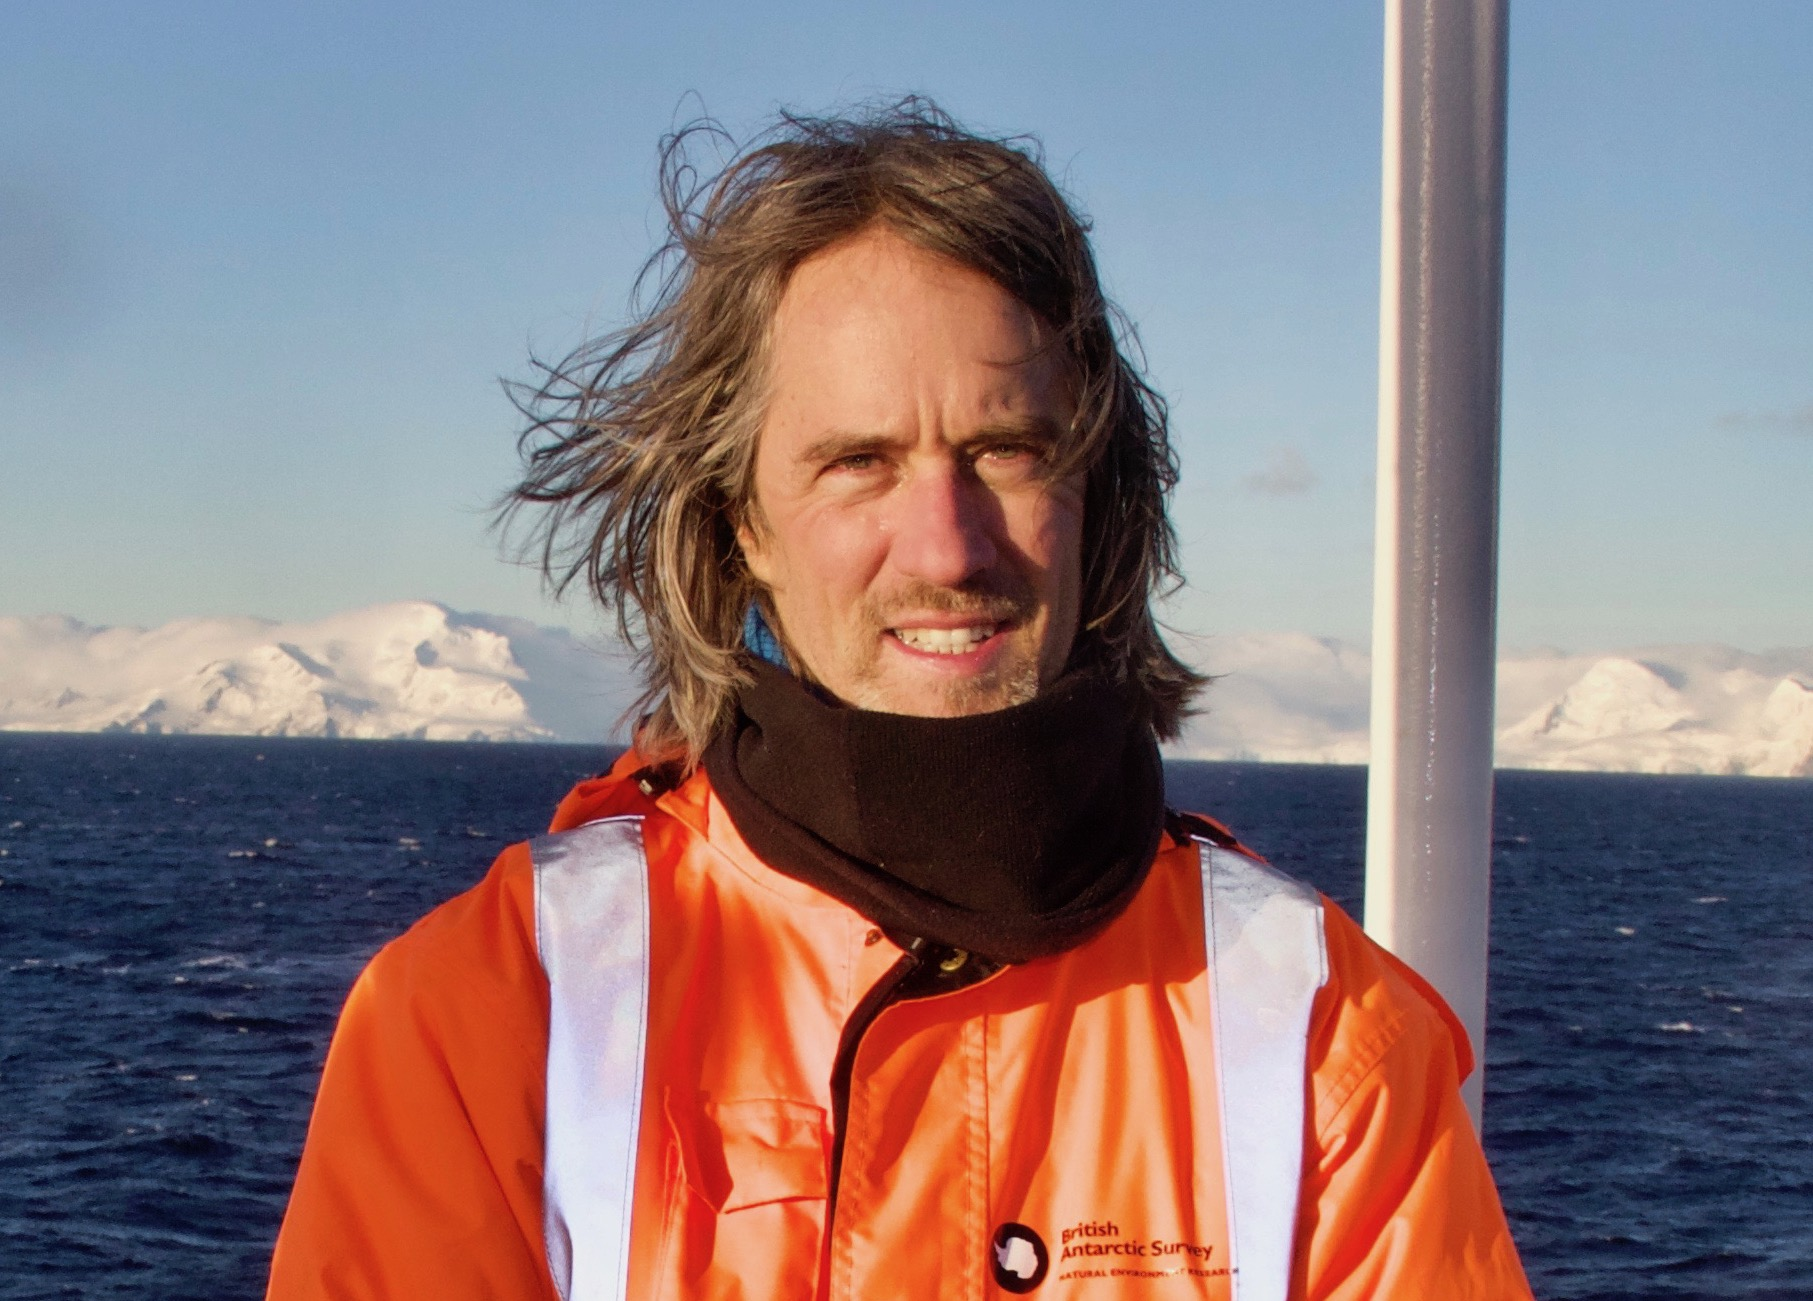
\includegraphics{Griffies_Coronation_Island_2017_crop.jpg}}

%\resizebox{2.5cm}{!}{\includegraphics{Griffies_photo_2021.jpeg}}

%\end{center}

\textsc{\large \color{Maroon} \protect Stephen Matthew Grif\/f\/ies (he/him/his)}
\\[1ex]

NOAA Geophysical Fluid Dynamics Laboratory (GFDL)
%$\bullet$ Princeton USA
\\
Princeton University Program in Atmospheric and Oceanic Sciences 
\\
{\tt \small Stephen.Griffies at noaa.gov} $\bullet$
{\tt \small  SMG at Princeton.edu} 
$\bullet$ {\tt  \small Stephen.M.Griffies at gmail.com} 
\\  
\vspace{0.1cm}

\href{https://StephenGriffies.github.io/}{research and teaching \hspace{0.5cm}}
\href{https://orcid.org/0000-0002-3711-236X}{orcid \hspace{0.5cm}}
\href{https://scholar.google.com/citations?user=4LPPPBAAAAAJ&hl=en}{google scholar \hspace{0.5cm}}
\href{https://www.webofscience.com/wos/author/record/55160}{Web of Science}
\noindent\rule{\textwidth}{1pt}


%$\bullet$ 
%\href{https://scholar.google.com/citations?user=4LPPPBAAAAAJ&hl=en}{google scholar page}
%\\
%Princeton USA

%\vspace{.2cm}
\end{center}
%}


\vspace{-1cm}
\section*{\sc \color{Maroon}  employment and appointments} 
\vspace{-.25cm}
\begin{tabular}{ll}

2020--2024 & Team lead for the GFDL Ocean/Cryosphere Division's high resolution climate model project
  \\
  2015--present & Faculty member of Princeton University's Atmospheric and Oceanic Sciences Program
  \\
  2013--2017  & Member, GFDL Model Development Team Steering Committee  \\
  
  Jun-Aug 2012  & Visiting Scientist, National Center for Atmospheric
                  Research, Boulder, USA \\
  Jan-Jun 2011   & Distinguished Visiting Scientist Fellow, CSIRO Marine and Atmospheric Research, Hobart, Australia \\
  2011-present & Senior Scientist at GFDL (equivalent to university professor) \\ 
  Mar 2009         & Visiting Professor, Universite catholique de Louvain, Belgium \\
  Jan-Nov 2005   & Visiting Scientist, CSIRO Marine and Atmospheric  Research, Hobart, Australia \\
  2001--2005     & Leader of the GFDL Oceans and Climate Group \\
  2000--2011     & Co-lead of the GFDL Ocean Model and Climate Model Development Teams \\
  1996-present   &  Staff Physical Scientist, NOAA/GFDL \\  
\end{tabular}

\noindent\rule{\textwidth}{1pt}
\vspace{-1cm}
\section*{\sc \color{Maroon} education}
\vspace{-.25cm}
\begin{tabular}{lll}
1995-1996  &  Postdoctoral fellow in oceanography/climate (mentor: Kirk Bryan) & Princeton University 
\\
1993-1995  &  NOAA Climate and Global Change Fellow (mentor: Kirk Bryan) & Princeton University 
\\
1988-1993  &  PhD in theoretical physics 
(advisor: Mirjam Cveti\v{c}) 
& University of Pennsylvania 
\\
1987-1988  &  pre-PhD studies in physics & University of Washington
\\
1986-1987  &  Masters in engineering sciences \& applied mathematics   & Northwestern University\\
1981-1986  &  Bachelor of science in chemical engineering  & Louisiana State University \\
%1978-1981  & High school diploma  & Biloxi High School, Biloxi, Mississsippi
 \end{tabular}

\noindent\rule{\textwidth}{1pt}
\vspace{-1cm}
\section*{\sc  \color{Maroon}   awards and honors}
\vspace{-.25cm}

\begin{tabular}{ll}
  2022 & NOAA Administrator's Award (with 26 others) "For advancing the understanding of the Earth System \\ & by developing and applying NOAA's state-of-the-art Coupled Carbon-Chemistry-Climate model"
  \\
  2019 & Department of Commerce Silver Medal Award (with Robert Hallberg and Matthew Harrison): "For \\ &  developing the state-of-the-art Modular Ocean Model version 6 (MOM6) to strengthen the Nation's \\& longer-range environmental prediction capabilities."
  \\
  2017 & \href{https://eos.org/agu-news/celebrating-the-2017-class-of-fellows}{Elected Fellow of the American Geophysical Union} "For exceptional and sustained contributions to the \\ &  understanding of large-scale ocean circulation and physics and seminal advances in ocean modeling"
\\
  2017 & NOAA Administrator's Award (with Robert Hallberg) "For scientific leadership for the innovation \\ & of the versatile  community-based Modular Ocean Model MOM6" 
  \\
  2014 & \href{http://www.egu.eu/awards-medals/fridtjof-nansen/2014/stephen-m-griffies/}{European Geosciences Union Fridtjof Nansen Medal for
         Oceanographic Research}  "For 
outstanding \\ & contribution and leadership in 
ocean general circulation model development 
and critical insights in the \\ & physical 
nature and parameterization of ocean processes"
\\
  2013 & Department of Commerce Silver Medal Award (with nine other
  GFDL staff scientists): 
  "For development \\ & and application of NOAA's first comprehensive  
  Earth System Model  
  that couples the carbon cycle and \\ & climate for projection of changes" \\
  2012 & NOAA Administrator's Award "For scientific vision, leadership
  and development of 
  the Modular Ocean \\ & Model (MOM4) for climate modeling, research and
  predictions" \\
  2011 & CSIRO Distinguished Visiting Scientist Fellow, Australia \\
  2009 & Visiting Professor, Universite catholique de Louvain, Belgium\\
  97,99,01 & NOAA/Oceanic and Atmospheric Research Outstanding Scientific
  Review Paper\\
  1999 & NOAA/Oceanic and Atmospheric Research Outstanding Scientific Paper
\end{tabular}

\noindent\rule{\textwidth}{1pt}
\vspace{-1cm}
\section*{\sc \color{Maroon}  oceanographic field work}
\vspace{-.25cm}

%\begin{tabular}{l}
\begin{itemize}[leftmargin=*]
 \item 
 Mar-May 2017: Eight week cruise on the {\it RRS JC Ross}  to the Orkney Passage and Scotia Sea,
  as part of the
  Dynamics of the Orkney Passage Outflow (DynOPO) project. Principal Scientific Officer: A.\ Naveira Garabato. 
 \item 
  Jul 1993: Two week cruise on the {\it CCGS Hudson} to the Labrador Sea in support of  the WOCE Line AR7W Atlantic Circulation Experiment. Chief Scientist: J.\ Lazier.
\end{itemize}
%%\end{tabular}

\vspace{-.4cm}
\noindent\rule{\textwidth}{1pt}
\vspace{-1cm}
\section*{\sc  \color{Maroon}  university teaching}
\vspace{-.3cm}

\begin{itemize}[leftmargin=*]

\item Princeton University Atmospheric and Oceanic Sciences 572: Waves, instabilities, and turbulence in the atmosphere and ocean (24 lectures covering the full course and taught every year since 2014). 

\item Princeton University Atmospheric and Oceanic Sciences 571: Geophysical Fluid Dynamics (24 lectures covering the full course and taught 2023, 2024).

\end{itemize}




\vspace{-.4cm}
\section*{\sc  \color{Maroon}  professional services}
\vspace{-.25cm}

\begin{tabular}{ll}

2021-present & Editor-in-Chief for  AGU's  \href{http://agupubs.onlinelibrary.wiley.com/hub/journal/10.1002/(ISSN)1942-2466/editorial-board/editorial-board.html}{Journal of Advances in Modeling Earth Systems (JAMES)} 
 \\
 2020-2022 & Member of the Princeton University AOS Diversity, Equity, Inclusion, and Accessibility committee
 \\
2018-2020 & Ocean/Cryosphere Editor for AGU's  \href{http://agupubs.onlinelibrary.wiley.com/hub/journal/10.1002/(ISSN)1942-2466/editorial-board/editorial-board.html}{Journal of Advances in Modeling the Earth System (JAMES)} 
  \\
2014-2018 &  Member  WCRP/CLIVAR Scientific Steering Group \\
2012-2014     & CLIVAR/CliC/SCAR Southern Ocean Region Implementation Panel \\
2012-present &  \href{http://www.clivar.org/clivar-panels/omdp}{WCRP/CLIVAR Ocean Model Development Panel} ex-officio member
\\
2007-2018 & Editor of the journal {\bf Ocean Modelling} \\
2006-2009     &  WCRP/CLIVAR Scientific Steering Group (ex officio) \\
2004-2009     &  WCRP/CLIVAR Working Group on Coupled Modelling (ex officio) \\
1999-2012     & WCRP/CLIVAR Working Group on Ocean Model Development  (co-chair 2004-2009) \\
\end{tabular}


\noindent\rule{\textwidth}{1pt}
\vspace{-1cm}
\section*{\sc  \color{Maroon} mentoring and sabbatical hosting}
\vspace{-.25cm}

\begin{itemize}[leftmargin=*]

\item {\sc sabbatical hosting}: Jan Zika (UNSW, Aus), Hussein Aluie (Un of Rochester), Laure Zanna (Oxford, UK), Jianjun Yin (Un of Arizona), Terrence O'Kane (CSIRO, Hobart, Aus), {R\"{u}diger} Gerdes (AWI, Bremerhaven, Germany)

\item {\sc postdocs}: Wenda Zhang, Jan-Erik Tesdal, Hemant Khatri, Graeme MacGilchrist, Brandon Reichl, Amanda O'Rourke, Ivy Frenger, Adele Morrison, Carolina Dufour, Yalin Fan, Harper Simmons, Shafer Smith

\item {\sc graduate students}: Matthew Lobo, Houssam Yassin, Michael Bates (UNSW), 

\item {\sc interns}: Rachel Pang, Ruth Moorman, Benjamin Taylor, Nathaniel Tarshish, Henri Drake 

\end{itemize}

\vspace{-.5cm}
\noindent\rule{\textwidth}{1pt}

\vspace{-.75cm}

\section*{\sc \color{Maroon} papers related to application}

\small 

\vspace{-.25cm}
%\begin{etaremune}
\begin{enumerate}[leftmargin=*]


\item A new conceptual model of global ocean heat uptake, 2023:  J. M. Gregory, J.S. Bloch-Johnson, M.P. Couldrey, E. Exarchou, S.M. Grif\/f\/ies, T. Kuhlbrodt, E. Newsom, O.A. Saenko, T. Suzuki, Q. Wu, S. Urakawa, and L. Zanna, {\it accepted by Climate Dynamics}, doi:10.1007/s00382-023-06989-z
 
\item Importance of the Antarctic Slope Current in the Southern Ocean response to ice sheet melt and wind stress change, 2022: R.L. Beadling, J.P. Krasting, S.M. Grif\/f\/ies, W.J. Hurlin, B. Bronselear, J.L. Russell, G. A. MacGilchrist, J.-E. Tesdal, M. Winton, {\it JGR-Oceans}, {\bf 127}, e2021JC017608, doi:10.1029/2021JC017608

\item A potential energy analysis of ocean surface mixed layers, 2022: B. Reichl, A. Adcroft, S.M. Grif\/f\/ies, and R.W. Hallberg, {\it JGR-Oceans}, {\bf 127}, e2021JC018140, doi:10.1029/2021JC018140

\item What causes the spread of model projections of ocean dynamic level change in response to greenhouse gas forcing?, 2021:  M.P. Couldrey, J.M. Gregory,  F. Boeira Dias, P. Dobrohotoff, C. Domingues, O. Garuba, S.M. Griffies, H. Haak, A. Hu, M. Ishii, J. Jungclaus, A. {K\"{o}hlaffil}, S. Marsland, S. Ojha, O.A. Saenko, A. Savita, A. Shao, D. Stammer, T. Suzuki, A. Todd, L. Zanna, {\it Climate Dynamics}, doi:10.1007/s00382-020-05471-4

\item Contribution of ocean physics and dynamics at different scales to heat uptake in low-resolution AOGCMs, 2020: O. Saenko, J.M. Gregory, S.M. Grif\/f\/ies, and F.\ Boeira Dias, {\it Journal of Climate}, doi:10.1175/JCLI-D-20-0652.1

\item Role of ocean model formulation in climate response uncertainty, 2019: J.P. Krasting, R.J. Stouffer, S.M. Grif\/f\/ies, R.W. Hallberg, S.L. Malyshev, B.L. Samuels, and L.T. Sentman, {\it Journal of Climate}, {\bf 31}, 9313-9333, doi:10.1175/JCLI-D-18-0035.1.

\item Change in future climate due to Antarctic meltwater, 2018: B. Bronselaer, M. Winton, S.M. Grif\/f\/ies, R.J. Stouffer, W.J. Hurlin, O.V. Sergienko, K. Rodgers, J. Russell, {\it  Nature}, doi:10.1038/s41586-018-0712-z.

\item The Flux-Anomaly-Forced Model Intercomparison Project (FAFMIP) for investigation of sea-level and ocean climate change in response to CO2 forcing, 2016: J. Gregory, N. Bouttes-Mauhourat, S.M. Grif\/f\/ies, H. Haak, W.J. Hurlin, J.  Jungclaus, M. Kelley, W.G. Lee, J. Marshall, A. Romanou, O.A. Saenko, D. Stammer, and M.  Winton, {\it Geoscientific Model Development},
  {\bf 9}, 3993--4017, doi:10.5194/gmd-9-3993-2016.

\item Mechanisms of Southern Ocean heat uptake and transport in a global eddying climate model, 2016: A.K. Morrison, S.M. Grif\/f\/ies, M. Winton, W.G. Anderson, and J.L. Sarmiento, {\it Journal of Climate}, {\bf 29}, 2059--2075, doi:10.1175/JCLI-D-15-0579.1

\item Impacts on ocean heat from transient mesoscale eddies in a hierarchy of climate models, 2015: S.M. Grif\/f\/ies, M. Winton, W.G. Anderson, R. Benson, T.L. Delworth, C.O. Dufour, J.P. Dunne, P. Goddard, A.K. Morrison, A. Rosati, A.T. Wittenberg, J. Yin, and R. Zhang, {\it Journal of Climate}, {\bf 28}, 952-977, doi:10.1175/JCLI-D-14-00353.1.

\item Has coarse ocean resolution biased simulations of transient climate sensitivity?, 2014: M.  Winton, W.G. Anderson, T.L. Delworth, S.M. Grif\/f\/ies, W.J. Hurlin and A. Rosati, {\it Geophysical Research Letters}, doi:10.1002/2014GL061523.

\item The deep ocean buoyancy budget and its temporal variability,  2013: J.B. Palter, S.M. Grif\/f\/ies, E.D. Galbraith,  A. Gnanadesikan, B.L. Samuels, and A. Klocker, {\it Journal of Climate}, {\bf 27}, 551--573,   doi:10.1175/JCLI-D-13-00016.1.

\item Influence of ocean and atmosphere components on simulated climate sensitivities, 2013: M. Winton, A.J. Adcroft, S.M. Grif\/f\/ies, R.W. Hallberg, L.W. Horowitz and R.J. Stouffer, {\it Journal of Climate}, {\bf 26}, 231--245,  doi:10.1175/JCLI-D-12-00121.1.

\item Northern high latitude heat budget decomposition and transient warming, 2013: M.A.A. Rugenstein, M. Winton, R.J. Stouffer, S.M. Grif\/f\/ies, and R.W. Hallberg, {\it Journal of Climate}, {\bf 26}, 609-621, doi:10.1175/JCLI-D-11-00695.1.

\item Connecting changing ocean circulation with changing climate, 2012: M. Winton, S.M. Grif\/f\/ies, B.L. Samuels, J.L. Sarmiento, and T.L. Froelicher, {\it Journal of Climate}, {\bf 26}, 2268--2278, doi:10.1175/JCLI-D-12-00296.1.

\item Physical processes that impact the evolution of global mean sea  level in ocean climate models, 2012: S.M. Grif\/f\/ies and R. J.\  Greatbatch, {\it Ocean Modelling}, {\bf 51}, 37--72,  doi:10.1016/j.ocemod.2012.04.003.


%\end{etaremune}
\end{enumerate}


\end{document}
